\documentclass[12pt]{article}

\usepackage[hungarian]{babel}
\usepackage{t1enc}
\usepackage[utf8]{inputenc}
\usepackage[margin=2.5cm]{geometry}
\usepackage{setspace}
\usepackage{graphicx}
\usepackage{float}
\usepackage{hanging}
\PassOptionsToPackage{hyphens}{url}\usepackage{hyperref}

\hypersetup{
    colorlinks,
    citecolor=black,
    filecolor=black,
    linkcolor=black,
    urlcolor=blue
}

\graphicspath{ {./figs/} }
\setlength{\belowcaptionskip}{5pt plus 3pt minus 2pt}

\setstretch{1.5}

\begin{document}

\begin{titlepage}
	\begin{center}
		\vspace*{5cm}
		
		\Huge
		\textbf{Kockázatmodellezés és -előrejelzés}
		
		\vspace{2cm}
		
		\LARGE
		Salamon András, Szilágyi Gergő
		
		\vfill
		
		\Large
		Hitelek és kockázatok makro és mikro szinten \\

        \vspace{1cm}
        
        2023. tavaszi félév
            
    \end{center}
\end{titlepage}

\newgeometry{margin=2.5cm}

\tableofcontents

\clearpage

\listoffigures

\clearpage

\section{Historikus VaR}

A Value at Risk (VaR) egy mutató, amivel egy eszköz, vagy egy portfólió lehetséges veszteségét lehet számszerűsíteni. Azt mutatja meg, hogy adott konfidenciaintervallum mellett legrosszabb esetben mennyit veszítünk a befektetésünkkel. A VaR számtásának egyik módja a historikus VaR, amikor múltbeli adatokból indulunk ki. A feladatunk ennek kiszámtása volt egy kételemű portfólióra. Két ETF-et, a MOO-t és a VOO-t választottuk ehhez.

A két eszköznek összesen 100 féle súlyozását néztük meg, ami az egész $[0,1]$ intervallumot lefedte. Így megkaptuk azt az optimális súlyozást, ami a legjobb historikus VaR értéket adja.

\begin{figure}[H]
	\centering
	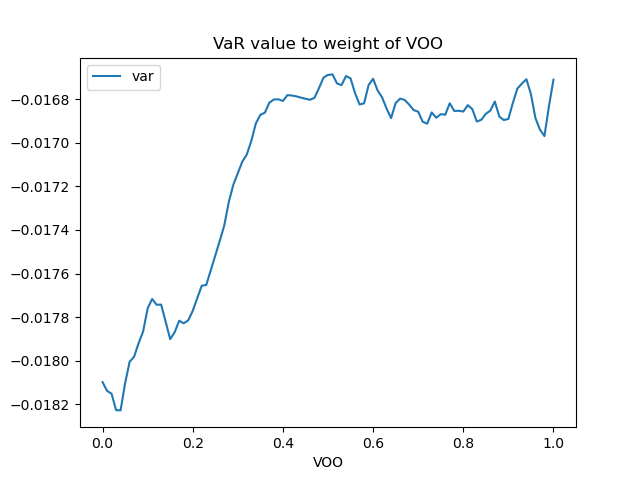
\includegraphics[scale=0.9]{var}
	\caption{VaR értéke a VOO súlyának függvényében, 95\%-os konfidencia szint mellett}
\end{figure}

Ahogy az ábrán az látható, kb. 0.2\%-os VaR eltérést tudunk elérni az eszközök optimális súlyozásával. A legmagasabb VaR érték -1,67\%, ez azt jelenti, hogy a hozamok 95\%-a ennél magasabb volt. Ehhez majdnem fele-fele arányban kell venni a két eszközt: a VOO súlya 0.51, a MOO-é 0.49.



\section{Szimulált VaR}



\section{EWMA}

Az EWMA (Exponentially Weighted Moving Average) segítségével szimulálható a pénzpiacokon megfigyelhető volatilitásklasztereződés. Eszerint azokat a napokat volatilisebb napok követik, amelyeken jobban ingadozik az árfolyam, valamint ez fordítva is igaz, a nyugodtabb napokat nyugodtabb napok követik. Az EWMA-ban az előző időszaki loghozamok négyzetét exponenciálisan csökkenő súlyokkal súlyozzuk. Az, hogy mennyire gyors az exponenciális csökkenés, a decay faktor értéke határozza meg. A súlyokat egyre normálva nagyobb decay faktor mellett kisebb súlyokat kapunk, azonban a súlyok lassabban csökkennek.

\begin{figure}[H]
	\centering
	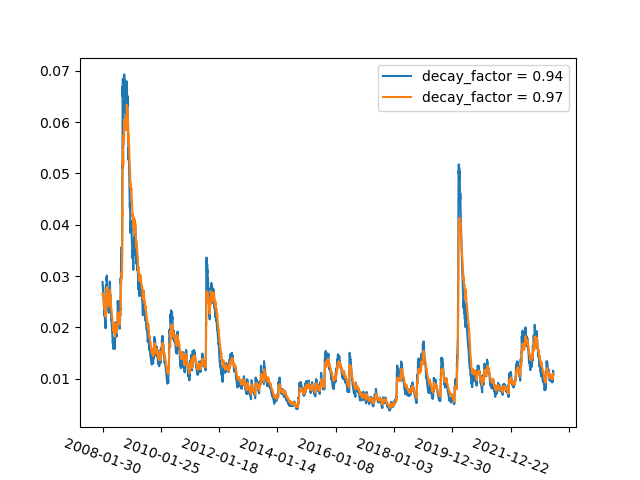
\includegraphics[scale=0.8]{ewma}
	\caption{EWMA a MOO idősoros adatokon a két decay faktor mellett}
\end{figure}

Ahogy az ábrán látható, nagyobb decay faktor mellett nagyobb az előrejelzett volatilitás, azonban ebben az esetben a volatilitások jobban klasztereződnek, mivel nem olyan nagyok a kilengések, mint kisebb decay faktor mellett.


\section{Machine Learning}

Végezetül készítettünk egy lineáris regressziós modellt is a jövőbeli variancia múltbeli adatokból történő előrejelzésére. A célváltozó az adott napi loghozam négyzete, a magyarázó változó pedig az előző 10 napi loghozamok négyzete, az EWMA módszeréhez hasonlóan. 

Az optimális fokszám megtalálásához hiperparaméter-keresést végeztünk, ennek az eredménye az lett, hogy a legalacsonyabb MSE az elsőfokú modell mellett volt. A cross-validation ezt az eredményt megerősítette. A végső modell koefficiensei a következőek: 
$$(0.1335, 0.0755, 0.0190, 0.0989, -0.0552; 0.0695, 0.0981, 0.0971, 0.0656, -0.0007).$$

Látható, hogy a legnagyobb koefficiens a legelső változóhoz, azaz az 1 nappal korábbi loghozamhoz tartozik. Ez megfelel a várakozásainknak. A korábbi napi adatokhoz tartozó koefficiensek azonban nem szabályosan csökkennek, így kétséges, hogy mennyire használható a modellünk. Ha nem csak bő 2 év adatait vizsgáljuk, és/vagy több napra visszamenően vesszük a magyarázó változókat, talán jobb modellt kaphatunk.

\end{document}














